%auto-ignore
\documentclass[preview=false]{standalone}

\usepackage{graphics,graphicx,xcolor}
\usepackage{standalone}
\usepackage{tikz}
\usetikzlibrary{automata, arrows.meta, positioning}

\definecolor{rouge}{RGB}{255,77,77}
\definecolor{vert}{RGB}{0,178,102}
\definecolor{jaune}{RGB}{255,255,0}
\definecolor{violet}{RGB}{208,32,144}
\definecolor{orange}{RGB}{255,140,0}
\definecolor{bleu}{RGB}{0,0,205}

 
\begin{document}
 
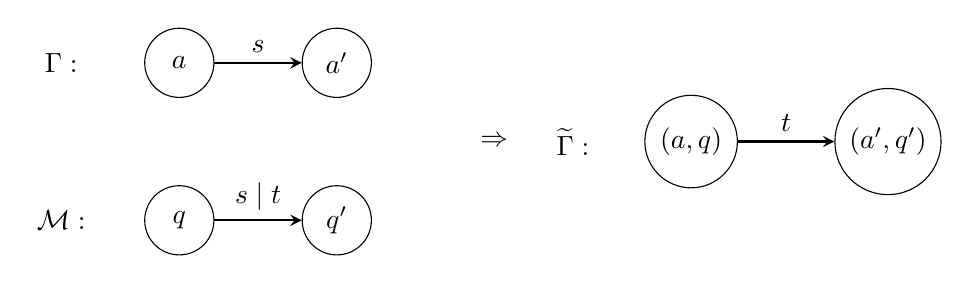
\begin{tikzpicture}[node distance = 3cm, on grid, auto]
    \node at (-1.5,0) {$\Gamma:$};
    \node (q0) [state] at (0,0) {$a$};
    \node (q1) [state] at (2,0) {$a'$};

    \node at (-1.5,-2) {$\mathcal{M}:$};
    \node (q2) [state] at (0,-2) {$q$};
    \node (q3) [state] at (2,-2) {$q'$};

    \node at (4,-1) {$\Rightarrow$};

    \node at (5,-1) {$\widetilde{\Gamma}:$};
    \node (q4) [state] at (6.5,-1) {$(a,q)$};
    \node (q5) [state] at (9,-1) {$(a',q')$};

\path [-stealth, thick]
    (q0) edge node {$s$}   (q1)
    (q2) edge node {$s\mid t$}   (q3)
    (q4) edge node {$t$}   (q5);

\end{tikzpicture}


\end{document}
